\makeatletter
\let\@starttocorig\@starttoc
\makeatother

\documentclass[oneside,20pt,fleqn,extrafontsizes]{memoir}

%%% color definition names: xcolor
\usepackage[usenames,dvipsnames]{xcolor}
\definecolor{bulgarianrose}{rgb}{0.28, 0.02, 0.03}
\definecolor{ashgrey}{rgb}{0.7, 0.75, 0.71}
\definecolor{red(ryb)}{rgb}{1.0, 0.15, 0.07}
\definecolor{wocrit}{rgb}{0.75, 0.25, 0.0}

%%% Import other packages%
\usepackage{usepkg}

%% import moodded thing
\usepackage{localF}
\usepackage{mathOp}
%%%%%%%%%%%%%%%%%% refname, titletoc, titlesec setting
\usepackage{titleT-ref}%toc depth

%%%%%%%%%%%% Hyperref package
\usepackage{hyperref}
\hypersetup{
    colorlinks,
    citecolor=black,
    filecolor=black,
    linkcolor=black,
    urlcolor=black
}

%%%%%%%%%%%%%%%%%%%%%%%%
%%%%%%%%%%%%%%%%%Geometry package
\usepackage{mygeometry}
%%%%%%%
\usepackage{fancypkg}%%%import fancy package with memoir correction

%%%%%%%%%%%%%%%%%% setlength
\usepackage{mylength}
\linespread{0.5}

%%%%%%% META
\title{Esami Settembre 19: l'Essenziale}

%%import makeidx
%\usepackage{makeidx}

%%% COUNTERS
\setsecnumdepth{subsection}
\setcounter{tocdepth}{-1}       % chapter
\newcounter{cherrychapter}%[chapte]
\setcounter{cherrychapter}{1}
\newcounter{partworkouts}%[chapte]
\setcounter{partworkouts}{1}

%%%% iimport functions
\usepackage{functions}
\usepackage{sources}
%%%%%%%%%%%%%%%%%%%% MULTINDExssss (number of chapters)
%\makeindex[1]%biasmomentumoggi]%chapters
%\makeindex[2]%meditazione]
%\makeindex[3]%nitidezza]
%\makeindex[4]%teatro]
\setsecnumdepth{subsection}
\settocdepth{chapter}
 
\begin{document}%BEGIN
\pagestyle{mystyle}%% mystyle defined in usepkg
\renewcommand*{\contentsname}{\label{toc}{Table of Contents}}%%\printcontents without head/hypereff
%\makeatletter
%\renewcommand*{\@tocmaketitle}{\label{toc}{Table of Contents}}
%\makeatother
\maketitle
\startcontents[chapters]

\tableofcontents*

\part{Fisica nucleare}
\documentclass[main.tex]{subfiles}
 
\begin{document}

\chapter{BB nucleosynthesis}
\PartialToc

\section{Proton capture on light elements}

\begin{itemize}
\item $D(^1H,\gamma)^3He$,$T_D\approx \SI{1e6}{\kelvin}$
\item $^7Li(^1H,^4He)^4He$, $T_{Li}\approx\SI{3e6}{\kelvin}$ 

\end{itemize}

\chapter{Nuclear burning in stars}
\PartialToc

\section{neutrino production}
\begin{itemize}
\item  Pair annihilation $\Pelectron+\APelectron\to\Pnue+\APnue$: $T>\SI{e9}{\kelvin}$ prob \num{e-19}
\item Photoneutrino: $\gamma+\Pelectron\to\Pelectron+\APnue+\Pnue$ in compton scattering
\item plasma neutrino: $\gamma_p\to\Pnue+\APnue$ - fotone accoppiato al moto collettivo degli elettroni in gas densi ionizzati - fotone \'e detto plasmone con massa efficace $\frac{h\omega_p}{2\pi c^2}$
\item Inelastic scattering of electrons in coulomb field produce photons but at vh densities and low T \Pnue\APnue pair - large atomic number
\item URCA: $(Z,A)+\Pelectron\to(Z-1,A)+\Pnue\to(Z,A)+\Pelectron+\APelectron$
\end{itemize}
\section{Fusion}
\begin{align*}
&\TDy{t}{X_i}=-A_im_HR_{ij}\\
&=-\rho\frac{X_iX_j}{m_HA_j}\frac{\exv{\sigma v}_{ij}}{1+\delta_{ij}}
\end{align*} 

\section{H burning: pp chain}

\section{H burning: CNO cycle}

\section{He burning}

\section{C-burning}

\section{photo-disintegration}
same as photo-diss but nuclear binding energy (from C-burning): 

\end{document}
%\documentclass[main.tex]{subfiles}
 
\begin{document}

\section{Modello a Gas di Fermi del nucleo}
\tool{
\begin{enumerate}
\item Conversione eV Kelvin\\
\begin{align*}
1  ^{\degree}K&= 8.621738*10^{-5}  eV \\
&= 0.0862 meV \\
&= 0.695 cm^{-1}
\end{align*}
\begin{gather*}
     1 a.u=27.211396 eV=219474.63 cm^{-1}\\
     1 Ry=13.6057 eV \\
     1 eV =8065.54 cm^{-1} \\
     1 eV= 11,600  ^{\degree}K\\
   1 meV = 8.065 cm^{-1}\\
\end{gather*}

\item Particella confinata in una scatola di lato L\\
Condizioni al bordo cubo lato L: $k_iL=n_i \pi $ quindi $k^2=\frac{\pi^2}{L^2}(n_x^2+n_y^2+n_z^2)$.
Energia: $E=\frac{\hbar^2k^2}{2m}=\frac{\hbar^2\pi^2n^2}{2mL^2}$
\end{enumerate}
}

Since the nuclear density is almost constant over the nuclear volume we may approxmate the nucleus as a Fermi free gas confined in a well of nuclear dimension.

\subsection{Modello a gas di Fermi del  nucleo}
\textbf{Modello a particelle indipendenti}\\
N particelle identiche non interagenti: $H=\sum_i^N [ \frac{p_i^2}{2m}+V_{\inf}(r_i)]$.\\
\textbf{Zero temperature approx}:\\
The kinetic energy associated to localization in nuclear volume (few MeV) is large compared with room temperature ($\frac{1}{40} eV$).

\subsection{Calcolo della densit\'a degli stati per un sistema di N fermioni identici in una scatola}
Density of available state $\frac{dN}{4\pi p^2dp}$ is given by $dN=4*\frac{4\pi p^2\Omega}{h}dp$: we are allowed to place 4 particles in each orbital (spin-isospin).\\
\textbf{Spazio delle Fasi}\\
In un volume dello spazio delle fasi $(2\pi\hbar)^3$ ci stanno al pi\'u $\nu$ particelle dove $\nu$ \'e la degenerazione.\\
\textbf{Density of states}\\
Semi-Euristico (Numero di stati fratto volume dello spazio delgi impulsi)\\
Number of states between $p$ e $p+dp$ is given by $dN=4*\frac{d^3p}{(2\pi\hbar)^3}\Omega=4*\frac{4\pi p^2dp}{(2\pi\hbar)^3}\Omega$.\\
The infinitesimal thin spherical shell with radius $dp$ has the volume $4\pi p^2dp$.\\
$g(k)=\frac{dN}{4\pi p^2dp}=\nu\frac{\Omega}{(2\pi)^3}$.\\

\textbf{Stati particella in una scatola}\\
Sia il numero di stati tra $n$ e $n+dn$: $dN=\nu \frac{4\pi n^2dn}{8}$, dove $\nu$ \'e il fattore di degenerazione. La densit\'a di stati fra $k$ e $k+dk$ \'e $g(k)=\frac{dN}{4\pi k^2dk}=\nu \frac{V}{(2\pi)^3}$.\\
\ev{g(k)=\frac{dN}{4\pi k^2dk}=\nu \frac{V}{(2\pi)^3}}

\subsection{Relazione tra densit\'a dei nucleoni e impulso di Fermi}
$A=\int_0^{+\infty}g(k)n(k)4\pi k^2dk$, $n(k)$ \'e il numero medio di occupazione dei livelli di singola particella: per gas completamente degenere (T=0)    
 $n(k)=\theta (k_F-k)$. Quindi: $A=\int_0^{k_F}g(k)4\pi k^2dk=\nu \frac{V}{(2\pi)^3}4\pi \frac{k_F^3}{3}$, e la densit\'a dei nucleoni \'e\\
\ev{\rho =\frac{A}{V}=(\frac{3\pi^2\rho}{3})^{\frac{1}{3}}\nu \frac{k_F^3}{6\pi^2}}\\
dato che $\rho=\frac{A}{V}=\frac{A}{\frac{4\pi}{3}r_0^3A}$ ottengo \ev{K_F=(\frac{9}{8}\pi)^{\frac{1}{3}}\frac{1}{r_0}} $(\nu=4)$.
Sapendo che la densit\'a (centrale) $\rho=0,17 Nucleone/fm^3$ ricavo $K_F=(\frac{9}{8}\pi)^{\frac{1}{3}}(\frac{\frac{3}{\rho_0}}{4\pi})^{-\frac{1}{3}}=1,36 fm^{-1}$.

\subsection{Relazione fra densit\'a ed energia di Fermi:}
Energia di Fermi = energia dello stato occupato pi\'u alto: $\epsilon_F=\frac{\hbar^2k_F^2}{2m}\approx 38,35 MeV$ (Usando il $k_F$ della sezione di sopra).
Sostituendo l'espressione per $k_F$ ho: \ev{\epsilon_F=\frac{\hbar^2}{2m}\rho^{\frac{2}{3}}(\frac{6\pi^2}{\nu})^{\frac{2}{3}}}. 

\subsection{Energia cinetica per particella}
Determino l'energia media per nucleone:
$\epsilon_{Kin}=\frac{1}{2m_N}\frac{\int_0^{k_F}k^4dk}{\int_0^{k_F}k^2dk}=\frac{3}{5}\frac{p_F^2}{2m_N}$, o pi\'u direttamente \ev{\frac{E_{Kin}}{A}=\frac{3}{5}\epsilon_F \approx 24MeV}.\\
$\frac{E}{A}=- \frac{B}{A}=-a_V+\text{Trascuto gli altri termini}\approx-15 MeV$ ed essendo l'energia cinetica per particella $(\frac{E}{A})_{Cin}=24 MeV$ derivo che il potenziale di singola particella \'e $(\frac{E}{A})_{Pot}=-39MeV$.

\subsection{Relazione tra pressione e densit\'a}

\tool{
\begin{enumerate}
\item Potenziali termodinamici\\
$dF=-pdV-SdT$\\
$dG=Vdp-SdT$\\
$dU=-pdV+TdS$\\
$dH=Vdp+TdS$\\

\item Energia media per nucleone\\
$\frac{E_{Kin}}{A}=\frac{3}{5}\epsilon_F$

\item Pressione\\
P esercitata da un gas=Flusso medio di momento attraverso una superficie ideale unitaria.
$PV=\frac{1}{3}\int_0^{\infty}N(p)pv_pdp$ ($\exv{\vec{a} \cdot \hat{n}}=\frac{1}{3}a$)\\
\ev{P=-(\frac{\partial U}{\partial V})=N\frac{2}{5}\epsilon_F=\frac{2}{3}\frac{U}{V}}\\
Ricavo energia libera di Gibbs: $G=U+PV=N\epsilon_F$
\end{enumerate}
}

In maniera pi\'u meccanica $P=-\left.\frac{\partial E}{\partial V} \right|_{S,A}=-\frac{\partial (\frac{E}{A})}{\partial (\frac{V}{A})}=-\frac{\partial \epsilon}{\partial \frac{1}{\rho}}=\rho^2 \frac{\partial \epsilon}{\partial \rho}=\frac{2}{5}\frac{\hbar^2}{2m}(\frac{6\pi^2}{\nu})^{\frac{2}{3}}\rho^\frac{5}{3}$.

\subsection{(Calore specifico:Approssimazione)}
$\delta N=(\frac{\partial N}{\partial \epsilon})_{\epsilon_F}$: la quantit\'a fra parentesi \'e la densit\'a di stati alla superficie di Fermi e $\delta \epsilon \approx kT$ (Distrinuzione FD: approssimazione per basse temperature dello "slittamento" in avanti dei numeri di occupazione rispetto T=0) quindi l'energia per portare un gas di Fermi a temperatura $kT$ \'e: $\delta U\approx \delta NkT=g(\epsilon_F)(kT)^2 \Rightarrow C_v=(\frac{\partial U}{\partial T})_V=2g(\epsilon_F)k^2T=3(kN)\frac{T}{T_F}=3R\frac{T}{T_F}$ (Il risultato corretto \'e $C_V=k\frac{\pi^2}{3}g(\epsilon_F)kT=\frac{\pi^2}{2}R\frac{T}{T_F}$). 
The electronic degrees of freedom are largely "frozen out" at room temperature because it is not possible to excite the majority of electronics buried deep in the Fermi sea.

\subsection{Relazione fra termine di volume della SEMF e il modello a gas di Fermi}

This term arise from $\exv{T+V}$\\
\begin{itemize}
\item kinetic energy\\
$T=A*\exv{T}=\frac{3}{5}\frac{{P_F}^2}{2m_N}A=\frac{3}{5}\frac{\hbar^2}{2m_N}(\frac{3\pi^2\rho}{2})^{\frac{2}{3}}A$
\item Potential energy:\\
Central potential $V_C(r)$ between nucleons (other potential energy contibutions associated with the spins will tend to yield an average central potential when one integrates over all directions).\\
$V=\frac{1}{2}\sum_{ij}\int\rho(\vec{r_i})\rho(\vec{r_j})V_C(r_{ij})d^3r_id^3r_j\rightarrow$\\
we consider the potential between two nucleons and multiply by number of couples (all nucleons are equivalent, the total wave function is antisymmetrized)\\
$\rightarrow\frac{A(A-1)}{2}\int\rho(\vec{r_1})\rho(\vec{r_2})V_C(r_{12})d^3r_1d^3r_2$.\\
Since nucleon's density is constant over nuclear volume  $\Omega$ we estimate $\rho(\vec{r_i})=\frac{\text{Probability}}{\text{unit volume(see normalization)}}\approx\frac{1}{\Omega}$, $V_C$ is short-ranged and nuclear medium is uniform  the integration over $d^3r_2$,  $\int\rho(\vec{r_2})V_C(r_{12})d^3r_2\approx\frac{1}{\Omega}\int V_C(\vec{r})d^3r=\frac{\overline{V_C}}{\Omega}$, is indipendent of the location of 1.\\
 $V\approx\frac{A^2}{2\Omega}\overline{V_C}=\frac{1}{2}A\rho\overline{V_C} $ ($<0$ for attractive forces).\\
\ev{a_V=-\frac{T+V}{A}\approx c_2\rho-c_1\rho^{\frac{2}{3}}}, con $c_1$ associated with kinetic energy and $c_2$ with potential energy (The nuclei don't collapse: we don't considere the repulsive core).
\end{itemize}

\subsection{Relazione fra termine di superficie (SEMF) e il modello a gas di Fermi}

\begin{enumerate}
\item Finite Fermi gas on kinetic energy\\
The energy eigenfunction for cubic box $L^3$ (the shape change the result by a geometrical factor)  are $\psi=\sin{(k_xx)}\sin{(k_yy)}\sin{(k_zz)}$, but the state $k_i=0$ are not allowed; the number of states for $k_x=0$: $dN_x=4*\frac{L^2dk_ydk_z}{(2\pi)^2}=\frac{4S2\pi kdk}{6(2\pi)^2}=\frac{S}{3\pi}kdk$, con $S=6L^2$ superfice laterale del cubo.\\
\textbf{Correzione volume volume finito}: $dN=(\frac{2\Omega}{\pi^2}k^2-\frac{S}{\pi}k)dk$.
$A=\int_0^{k_F}(\frac{2\omega}{\pi^2}k^2-\frac{S}{\pi}k)dk=\frac{2\Omega}{3\pi^2}{k_F}^3-\frac{S}{2\pi}k_F^2=\frac{2\Omega}{3\pi^2}k_F^3(1-\frac{3\pi}{4}\frac{S}{\Omega}\frac{1}{k_F})$\\
$\exv{T}=\frac{\hbar^2}{2m_N}\frac{\int_0^{k_F}(\frac{2\Omega}{\pi^2}-\frac{S}{\pi}k^3)dk}{A}\approx\frac{3}{5}\frac{\hbar^2k_F^2}{2m_N}[1+\frac{\pi}{8}\frac{S}{\Omega}\frac{1}{k_F}+\ldots]$\\
Since for nuclei we have $\frac{S}{\Omega}\approx\frac{4\pi r_0^2A^{\frac{2}{3}}}{\frac{4\pi}{3}r_0^3A}\approx\frac{3}{r_0A^{\frac{1}{3}}}$: $\exv{T}=\frac{3}{5}E_F+\frac{9}{40}E_F\frac{\pi}{r_0k_F}\frac{1}{A^{\frac{1}{3}}}$.\\
\ev{a_S(T)=\frac{9}{40}E_F\frac{\pi}{r_0k_F}\approx 18 MeV} (valid only to within a geometric factor like 2 or 3)\\

\item Finite Fermi gas on potential energy\\
The volume associated with the nuclear surface is a shell of thickness approximately equal to the range of the nuclear force: $\delta\Omega\approx4\pi R^2r_1$.\\
Sottraggo la correzione all'energia potenziale $V\approx\frac{1}{2}A\rho\overline{V_C}(1-\frac{d\Omega}{\Omega})=\frac{1}{2}A\rho\overline{V_C}-\frac{3}{2}\rho\frac{r_1}{r_0}A^{\frac{2}{3}\overline{V_C}}$.\\
$a_S(V)\approx\frac{3}{2}\rho\frac{r_1}{r_2}\overline{V_C}$ ($>0$ for attrattive force)\\
\textbf{For a square well potential}:\\
$V=\frac{1}{2}A\rho\overline{V_C}[1-\frac{9}{16}\frac{r_1}{R}+\frac{1}{32}(\frac{r_1}{R})^3]$.
\end{enumerate}

\subsection{Relazione fra termine Coulombiano della SEMF e il modello a gas di Fermi}
\textbf{Charge density}: $\rho_e=\frac{Z}{A}\rho e=\frac{Ze}{\Omega}$\\
\textbf{Coulomb energy}: $V_c=\frac{1}{2}\int\rho_e^2\frac{d^3r_1d^3r_2}{r_{12}}=\rho_e^2\int_0^R\frac{4\pi r^3}{3}\frac{4\pi r^2dr}{r}=\frac{4\pi}{3}\rho_e^24\pi\frac{R^5}{5}=\frac{3}{5}\frac{Z^2e^2}{R}=\frac{3}{5}\frac{Z^2e^2}{r_0}A^{-\frac{1}{3}}$ quindi:\\
\ev{a_C=\frac{3}{5}\frac{e^2}{r_0}\approx 0.71 MeV}

\subsection{Relazione fra termine di simmetria della SEMF e il modello a gas di Fermi}
Calcolo del termine di simmetria della formula semiempirica di massa mediante il modello a gas di Fermi del nucleo.

\tool{
\begin{enumerate}
\item Energia cinetica per nucleone\\
$\frac{E_{Kin}}{A}=\frac{3}{5}\epsilon_F$
\item Energia di Fermi\\
$\epsilon_F=\frac{\hbar^2}{2m}\rho^{\frac{2}{3}}(\frac{6\pi^2}{\nu})^{\frac{2}{3}}$
\item Total kinetic energy for $N=Z$\\
$T_0=A\frac{3}{5}\frac{\hbar^2}{2m_N}(\frac{3\pi^2\rho_0}{2})^{\frac{2}{3}}$
\item  Espansioni di Taylor al secondo ordine intorno a $x=\frac{1}{2}$ con $\delta x=x-\frac{1}{2}=\frac{Z-N}{A}$: \\
\lbt{x^{\frac{5}{3}}=\frac{1}{2^{\frac{5}{3}}} +\frac{5}{3}\frac{1}{2^{\frac{2}{3}}}\delta x+\frac{10}{9}2^{\frac{1}{3}}\frac{{\delta x}^2}{2}+o({\delta x}^4)=(\frac{1+\beta}{2})^{\frac{5}{3}}}{(1-x)^{\frac{5}{3}}=\frac{1}{2^{\frac{5}{3}}} -\frac{5}{3}\frac{1}{2^{\frac{2}{3}}}\delta x+\frac{10}{9}2^{\frac{1}{3}}\frac{{\delta x}^2}{2}+o({\delta x}^4)=(\frac{1-\beta}{2})^{\frac{5}{3}}}
\end{enumerate}
}

The nuclear force prefers $T = 0$, so nuclei with $Z = N$ are expected to have extra stability and so maximize the binding energy B. Let’s assume two Fermi gases consisting of Z protons and N neutrons. We will allow the relative number of protons and neutrons to vary but we will keep $A = Z + N$ fixed.
\textbf{Densities of the two components}:\\
$\rho_0=\frac{A}{V}$, $\rho_p=\frac{Z}{A}\rho_0\equiv x\rho_0$, $\rho_n=\frac{N}{A}\rho_0\equiv (1-x)\rho_0$, $A=Z+N$ costante.

$E_{Cin}=\frac{3}{5}(N\epsilon_F^N+Z\epsilon_F^P)=\frac{3}{5}\frac{\hbar^2}{2M}\frac{(3\pi)^\frac{2}{3}}{2}(N^{\frac{5}{3}}+Z^{\frac{5}{3}})=T_P+T_N=2^\frac{2}{3}T_0[x^\frac{5}{3}+(1-x)^\frac{5}{3}]$, che espando intorno a $x=\frac{1}{2}$, il pongo $\delta x=x-\frac{1}{2}=\frac{Z-N}{A}$ e ottengo l'approssimazione  \ev{T_P+T_N=T_0+\frac{5}{9}T_0(\frac{Z-N}{A})^2=T_0+a_{Sym}\frac{(N-Z)^2}{A}}.

quindi $(\frac{E}{N})_{Sym}=\frac{5}{9}(\frac{E}{N})=a_{Sym}\approx 12.8 MeV$. Ricavo il contributo del potenziale nucleare a $a_{Sym}$:
$(\frac{E_{Sym}}{N})_{Int}=a_{Sym}-(\frac{E}{N})_{Sym}\approx16 MeV$, sapendo che $a_{Sym}\approx20-30 Mev$.

\subsection{Mean Free Path of Nucleons}

\begin{comment}
Mean Free Path of Nucleons
A fundamental characteristic of any many-body system is the mean free path for collisions between constituent particles. A wide variety of evidence testifies to the fact that, in the nucleus, this mean free path is large compared to the distance between the nucleons and even, under many circumstances, is larger than the dimensions of the nucleus.
A very direct way to explore the nuclear opacity is provided by scattering experiments involving incident neutrons and protons. 
%Figure 2-3, p. 165 shows typical examples of the energy dependence of the total cross section for inter- action of neutrons with nuclei.
 For a system with a mean free path small com- pared to the radius, the total cross section would vary monotonically with energy, decreasing slowly over the eneirgy region considered, toward the limiting value 2nR ’. (For a discussion of general scattering theory as applied to nuclei, and for the estimate of cross sections for totally absorbing systems, see, for example, Blatt and Weisskopf, 1952, Chapter 8.) The pronounced variations in the observed cross sections must be attributed to the interference between the incident and transmitted waves, and thus establish the fact that the mean free path is at least comparable with the nuclear radius. (We later return to the more quantitative analysis of such scattering experiments (Sec. 2-4c); see also the discussion in connection with Fig. 2-3.)
The relatively long mean free path of the nucleons implies that the inter- actions primarily contribute a smoothly varying average potential in which the particles move independently. As a first approximation of heavy nuclei, we may neglect surface effects, and the resulting Fermi gas model provides a useful starting point for the discussion of many of the bulk properties of nuclei.
\end{comment}
\end{document}

\part{Fundamental interactions}\label{intfon}
\documentclass[main.tex]{subfiles}
 
\begin{document}

\chapter{Newtonian potential}
\PartialToc

\section{two-body}

\section{Hamiltonian}

\begin{align*}
&H(p,q)=\frac{1}{2\mu}(p_r^2+\frac{1}{r^2}p_{\beta}^2+\frac{1}{r^2\cos^2{\beta}}p_{\lambda}^2)-\frac{k^2\mu}{r}
\end{align*}


\section{perturbation}

\section{3-body}

\end{document}
\documentclass[main.tex]{subfiles}
 
\begin{document}

\chapter{astro plasma physics}
%\PartialToc

La presenza dello ione $Z_i$ altera la distribuzione di cariche quindi devo determinare il potenziale $\phi_i$ generato da $Z_i$ e dalla distribuzione di cariche attorno; usando la formula di Boltzmann la densit\'a delle particelle con carica Z risulta
\begin{equation}\label{eq:Bdistroelectricpot}
n_Z=\overline{n}_Z\exp{-\frac{Ze\phi}{kT}}
\end{equation}
con $\overline{n}_Z$ densit\'a numerica della particella di carica $Z$ in assenza di $Z_i$.

L'equazione di Poisson per $\phi$ \'e
\begin{equation}\label{eq:poissonscreened}
\nabla^2\phi=-4\pi e\sum_Z Zn_Z-4\pi e\sum_i Z_i\delta(\vec{r}-\vec{r}_i)
\end{equation}

Nel regime di schermaggio debole, dove l'energia coulombiana \'e molto minore dell'energia termica $e\phi\ll KT$, espando $n_Z$ (\eqref{eq:Bdistroelectricpot}) al prim'ordine quindi in \eqref{eq:poissonscreened} rimane il termine lineare in $\phi$.

Introduco il raggio di Debye:
\begin{equation}
\frac{1}{r_D^2}=\frac{4\pi e^2}{kT}\sum Z^2\overline{n}_Z=\frac{4\pi e^2}{kT}N_A\zeta,\ \zeta=\sum_{i}(Z_i^2+Z_i)\frac{\rho X_i}{A_i}\label{eq:debyeradius}
\end{equation}
quindi dall'equazione \eqref{eq:poissonscreened} ottengo il potenziale generato dallo ione $Z_i$ in $\vec{r}_i$ a distanza $|\vec{r}-\vec{r}_i|=r_i$ come soluzione di:
\begin{equation}\label{eq:poissonspheric}
\frac{r_D^2}{r_i}\TtwoDy{r_i}{(r_i\phi_i)}=\phi_i
\end{equation}
con
\begin{equation}
\phi=\sum_i\phi_i
\end{equation}

\begin{workout}[Raggio di debye e degenerazione elettronica]
Il rapporto fra densit\'a elettronica e quella imperturbata \'e
\begin{equation}
\midfrac{f(\psi-\midfrac{U_e(r)}{KT})}{f(\psi)}
\end{equation}
dove $U_e(r)$ \'e l'energia di interazione di un elettrone
\end{workout}

La soluzione di \eqref{eq:poissonspheric} \'e
\begin{equation}\label{eq:screenedpotential}
\phi_i=\frac{Z_ie}{r_i}\exp{-\midfrac{r}{r_D}}
\end{equation}


\chapter{opacity sources}
%\PartialToc

\section{Grain opacity in planetary gas accretion}
$\kappa_{gr}=\frac{Q(x)\pi a^2n_{gr}}{\rho}=\frac{3Q(x)f_{d/g}}{4\rho_{gr}a}$
If $a\gg\lambda$ $Q(x)\approx2$ with $x=2\pi a/\lambda$

\section{ISM dust}
%ism-ch3-dust.pdf
%Dust.pdf
%%vanderanker_slides.pdf
%Draine_IPMU_Lectures.pdf

\chapter{Evapopration ??}
%\PartialToc

Potential
\begin{align*}
&\chi(r)=-\frac{GM_p}{r}+C\\
&\chi'(r)=\chi(r)+\Delta\chi(r)=-G(M_p+M_*)[\frac{\mu}{r}+\frac{1-\mu}{a_p-r}+\frac{((1-\mu)a_p-r)^2}{2a_p^3}]+C\\
&\mu=\frac{M_p}{M_p+M_*}
\end{align*}
Energy needed to escape the planet $\PDy{r}{\chi'}|_{R_h}=0$

\section{Stellar spectrum}

FUV: $\SI{6}{\ev}\leq h\nu\leq\SI{13.6}{\ev}$
EUV: $\SI{13.6}{\ev}\leq h\nu\leq\SI{0.1}{\kilo\ev}$
X-rays: $h\nu\geq\SI{0.1}{\kilo\ev}$

\end{document}
\documentclass[main.tex]{subfiles}
 
\begin{document}

\chapter{Comportamento materia densit\'a temperature stellari}

\section{EOS}

\subsection{Fully ionized perfect gas}

\keyword{perfect gas}: potential energy between particle negligible respect kinetic energy and de Broglie $\lambda_{dB}=\frac{h}{p}\ll\lambda$ mean distance between particles - maxwell distro with mean kinetic energy $\frac{3}{2}kT$:
\begin{align*}
&kT>\frac{Z^2e^2}{d}\\
&\frac{4\pi}{3}nd^3=\frac{4\pi\rho}{3\mu m_H}d^3=1\\
&d\approx(\frac{\mu m_H}{\rho})\expy{1/3}\\
&\frac{h}{p}=\frac{h}{\sqrt{2mkT}}\ll d
\end{align*}
\keyword{Free energy per unit mass of perfect gas}:
\begin{align*}
&F=-kT\sum_sN_s[\frac{3}{2}\ln{T}-\ln{(N_s\rho)}+\ln{G_s}+1+\ln{g_s}]+F_{int}
\end{align*}
$g_s$ statistical weight (number of state with same energy), $G_s=(2\pi km_s/h^2)\expy{3/2}$, $F_{int}$ energia libera particelle con stati legati

\subsection{Non-ideal corrections: Interazione coulombiana}

Corrections parametrized by $\Gamma=\frac{(Ze)^2}{dkT}$: when density suff. low $\Gamma\approx0$; for fully ionized mixture
\begin{align*}
&\Gamma=\frac{\exv{Z}\expy{1/3}e^2}{d'kT}\exv{Z\expy{5/3}}\\
&d'=(\frac{4\pi\rho}{3\mu_im_H})\expy{-1/3}
\end{align*}
La principale correzione che tiene conto dell'interazioni tra particelle \'e dovuta alle interazioni coulombiane.

\begin{workout}[Correzioni interazioni coulombiane- vedi schermaggio]

\end{workout}

La presenza dello ione $Z_i$ altera la distribuzione di cariche quindi devo determinare il potenziale $\phi_i$ generato da $Z_i$ e dalla distribuzione di cariche attorno; usando la formula di Boltzmann la densit\'a delle particelle con carica Z risulta
\begin{equation}\label{eq:Bdistroelectricpot}
n_Z=\overline{n}_Z\exp{-\frac{Ze\phi}{kT}}
\end{equation}
con $\overline{n}_Z$ densit\'a numerica della particella di carica $Z$ in assenza di $Z_i$.

L'equazione di Poisson per $\phi$ \'e
\begin{equation}\label{eq:poissonscreened}
\nabla^2\phi=-4\pi e\sum_Z Zn_Z-4\pi e\sum_i Z_i\delta(\vec{r}-\vec{r}_i)
\end{equation}

Nel regime di schermaggio debole, dove l'energia coulombiana \'e molto minore dell'energia termica $e\phi\ll KT$, espando $n_Z$ (\eqref{eq:Bdistroelectricpot}) al prim'ordine quindi in \eqref{eq:poissonscreened} rimane il termine lineare in $\phi$.

Introduco il raggio di Debye:
\begin{equation}
\frac{1}{r_D^2}=\frac{4\pi e^2}{kT}\sum Z^2\overline{n}_Z=\frac{4\pi e^2}{kT}N_A\zeta,\ \zeta=\sum_{i}(Z_i^2+Z_i)\frac{\rho X_i}{A_i}\label{eq:debyeradius}
\end{equation}
quindi dall'equazione \eqref{eq:poissonscreened} ottengo il potenziale generato dallo ione $Z_i$ in $\vec{r}_i$ a distanza $|\vec{r}-\vec{r}_i|=r_i$ come soluzione di:
\begin{equation}\label{eq:poissonspheric}
\frac{r_D^2}{r_i}\TtwoDy{r_i}{(r_i\phi_i)}=\phi_i
\end{equation}
con
\begin{equation}
\phi=\sum_i\phi_i
\end{equation}

\begin{workout}[Raggio di debye e degenerazione elettronica]
Il rapporto fra densit\'a elettronica e quella imperturbata \'e
\begin{equation}
\midfrac{f(\psi-\midfrac{U_e(r)}{KT})}{f(\psi)}
\end{equation}
dove $U_e(r)$ \'e l'energia di interazione di un elettrone
\end{workout}

La soluzione di \eqref{eq:poissonspheric} \'e
\begin{equation}\label{eq:screenedpotential}
\phi_i=\frac{Z_ie}{r_i}\exp{-\midfrac{r}{r_D}}
\end{equation}

[formula corretta potenziale elettrostatico generato da nuvola elettronica attorno a $Z_i$]

\begin{align*}
&\nabla^2V_i=-4\pi e\sum Zn_Z\approx\frac{1}{r_D^2}V_i\intertext{da cui ottengo il potenziale generato dalla nube di cariche attorno a Z}
&\phi_Z=-\frac{eZ}{r_D}
\end{align*}
con $r_D$ raggio di Debye definito da:
\begin{equation*}
\frac{1}{r_D^2}=\frac{4\pi e^2}{kT}\sum Z^2\overline{n}_Z=\frac{4\pi e^2}{kT}N_A\zeta,\ \zeta=\sum_{i}(Z_i^2+Z_i)\frac{\rho X_i}{A_i}\label{eq:debyeradius}
\end{equation*}

[correzioni $u_c/P_c$: notazione consistente.]
Le correzioni dovute alle interazioni coulombiane sono
\begin{align}
&u=\frac{3}{2}\frac{\gasconstant{}T}{\mu}+u_c,\ \rho u_c=\frac{1}{2}\sum_ZeZ\overline{n}_Z\phi_Z=-e^3\sqrt{\frac{\pi\rho}{kT}}(N_A\zeta)\expy{\frac{3}{2}}\\
&P=\frac{\rho}{\mu}kT+P_c,\  P_c=\frac{1}{3}u_c
\end{align}

Le correzioni dovute alle interazioni coulombiane sono
\begin{align}
&u=\frac{3}{2}\frac{\gasconstant{}T}{\mu}+u_c,\ \rho u_c=\frac{1}{2}\int\phi(\vec{r})\rho_c(\vec{r})\,d^3r\\
&P=\frac{\rho}{\mu}kT+P_c,\  P_c=\frac{1}{3}\rho u_c
\end{align}

\section{Ordini di grandezza}

\subsection{Misure adimensionali interazioni}

Potenziale tra 2 nucleoni $-Gm_H^2/r$ con $r=\frac{h}{2\pi m_Hc}$ (Pindet): in unit\'a $m_Hc^2$ $\alpha_G=\frac{2\pi Gm_H^2}{hc}\approx\num{e-39}$.

$\alpha_{SF}=\frac{e^2}{(4\pi\epsilon_0)\hbar c}$.

The ratio of three characteristic lengths:

the classical electron radius $r_e=(\frac{1}{4\pi\epsilon_0})\frac{e^2}{m_ec^2}$, the Bohr radius $a_0=(4\pi\epsilon_0)\frac{\hbar^2}{m_ee^2}$  and the Compton wavelength of the electron $\lambdabar_e=\frac{\hbar}{m_ec}$:

$r_e=\frac{\alpha\lambda_e}{2\pi}=\alpha^2a_0$.

$e^2=1.44\,MeV\,fm$

TODO: pressure ionizzation and electron degeneracy (why eos for H,He)

\section{neutrino processes}

\end{document}

\part{Analisi statistica dati}\label{asd}
\documentclass[main.tex]{subfiles}
 
\begin{document}

\chapter{Probability and statistics}

\section{Kolmogorov axioms}
$X_i$ elementary events mutually exclusive
\begin{align*}
&\prob{(X_i)}\geq0,\ \forall i\\
&\prob{(X_i\cup X_j)}=\prob{(X_i)}+\prob{(X_j)}\\
&\sum_{\Omega}\prob{(X_i)}=1
\end{align*}
A, B insiemi di eventi elementari $X_i$ non esclusivi, $\prob{(A|B)}$ \'e prob. che evento elementare che appartiene a B sia anche in A
\begin{align*}
&\prob{(A\cap B)}=\prob{(A|B)}\prob{(B)}=\prob{(B|A)}\prob{(A)}
&\prob{(A\cup B)}=\prob{(A)}+\prob{(B)}-\prob{(A\cap)} 
\end{align*}
\begin{itemize}
\item Eventi indipendenti: joint probability equals product of probability
\begin{align*}
&\prob{(A\cap B)}=\prob{(A)}\prob{(B)}\Leftrightarrow \prob{(A)}\\
&=\frac{\prob{(A\cap B)}}{\prob{(B)}}=\prob{A|B}
\end{align*}
\item teorema probabilit\'a totale: $A\cap B=\emptyset$, $\prob{(A\cup B)}=\prob{(A)}+\prob{(B)}$
\item disuguaglianza di Chebychev: X ha media $\mu$ e var $\sigma^2$ e $\lambda>0$:
\[\prob{(|X-\mu|<\lambda\sigma)}\geq1-\frac{1}{\lambda^2}\]

\end{itemize}

\end{document}
\documentclass[main.tex]{subfiles}
 
\begin{document}

\chapter{inference}
\PartialToc

\section{Sufficiency}

\subsection{Statistica sufficiente}
\keyword{stat suff}: A statistic T is called sufficient for unknown parameter $\theta$ iff the conditional pdf of iid RV $X_1,\ldots,X_n$ dato $T=t$ don't involve $\theta$. Ex: \iidrv{X} Bernoulli p. $T=\sum_iX_i$ \'e suff: $\prob{(X_1=x_1\cap\ldots\cap X_n=x_n|T=t)}=0$ se $\sum_ix_i\neq t$; $A=\{\cap_iX_i=x_i\}\subseteq B=\{T=t\}$:
\begin{align*}
&\prob{(\cap_iX_i=x_i|T=t)}\\
&=\prob{(\cap_iX_i=x_i\cap T=t)}/\prob{(T=t)}\tag*{P condizionata}\\
&=\prob{(\cap_iX_i=x_i\cap T=t)}/\prob{(T=t)}\tag*{sottoinsieme di $T=t$}\\
&=\prod_i\prob{(X_i=x_i)}/\prob{(T=t)}\tag*{X's independent}
\end{align*}
quindi
\begin{align*}
&\prob{(\cap_iX_i=x_i|T=t)}\\
&=\frac{p\expy{\sum_ix_i}(1-p)\expy{n-\sum_ix_i}}{\binom{n}{t}p^t(1-p)\expy{n-t}}\\
&=1/\binom{n}{t}
\end{align*}
\subsection{T. fattorizzazione Neyman}
iid RV \iidrv{X} pdf $f(x;\theta)$, likelihood $L(\theta)=\prod_if(x_i;\theta)$. $T(X_1,\ldots,X_n)$ \'e suff per $\theta$ iff
\begin{equation*}
L(\theta)=g(T(x_1,\ldots,x_n);\theta)h(x_1,\ldots,x_n)
\end{equation*}
$A=\{X=x\}\subseteq B=\{T(X)=T(x)\}$; only if:
\begin{align*}
&L(\theta)=P_{\theta}(X=x)\\
&=P_{\theta}(X=x\cap T(X)=T(x))\\
&=\underbrace{P_{\theta}(T(X)=T(x))}_{g(T(x_1,\ldots,x_n);\theta)}\underbrace{P_{\theta}(X=x|T(X)=T(x))}_{h(x_1,\ldots,x_n)}
\end{align*}
If part pg 315

\section{Fisher Information}

\subsection{Score statistics}

\begin{align*}
&S=\PDy{\theta}{\log{L}}\\
&\E{[S]}=0\\
&\var{[S]}=-\E{[\PtwoDy{\theta}{\log{L}}]}=-I\\
&S\to N(0,I)
\end{align*}

Informazione di Fisher
\[I_{\Vec{X}}(\theta)=NI_{X_1}=N\E_{\theta}[(\PDy{\theta}\log{f(X_1;\theta)})^2]=-N\E_{\theta}[\PtwoDy{\theta}\log{f(X_1;\theta)}]\]
$I_{X}\geq I_T$ uguaglianza vale per T suff.

\section{Propriet\'a stimatori}

\begin{itemize}
\item consistenza: (LGN) $\E{(\hat{\theta})}\to\theta_0$
\end{itemize}

\section{Stimatori e caratteristiche patametri pdf: gaussian, poissonian, binom - unif}

MVB:

\section{Stimatore MLE di varianza segnale gaussiano con rumore gaussiano}

statistica suff: $s^2=\sum_ix_i^2$
stima mle $\hat{\sigma}^2=\max{(s^2/N-\sigma_0,0)}$.

$Y=\alpha X+b$ $\phi_Y(t)=$

var usando funzione GM della gaussiana
(momento n=2 integrato da $N\sigma_0$
(CRC PRESS 2000, pg 408)

\end{document}
\section{Test ipotesi e GOF}


\part{Evoluzione componente solida in dischi protoplanetari}\label{ppd}
\begin{frame}{Accrescimento dei planetesimi: collisioni.}
\begin{itemize}
\item $r_{pl}<b<\frac{Gm_{pl}}{v_r^2}=b_0$: incontro ravvicinato ($|U_{max}|>E_{kin}^{\infty}$ l'energia potenziale nel momento di massima interazione sovrasta energia cinetica a infinito).
\item $b>(\frac{m_{pl}}{3\msun{}})\expy{\frac{1}{3}}a=d_{Hill}$: passaggio a grande distanza.
\item $b_0<b<d_{Hill}$: deflessioni di direzione e verso casuali.
\end{itemize}
\begin{block}{Scattering $b>r_{pl}$: variazione velocit\'a relativa}
\begin{equation*}
\delta v_r=\underbrace{\frac{Gm_{pl}}{b^2}}_{\exv{a}}\underbrace{\frac{2b}{v_r}}_{\exv{\tau_{int}}}=\frac{2Gm_{pl}}{bv_r}
\end{equation*}
\end{block}
\begin{equation*}
b_0<b<d_{Hill}:\quad [\TDy{t}{v_r^2}]_{enc}=\int_{r_{pl}}^d2\pi bv_r\frac{\sigma n}{m_{pl}v_r}(\frac{2Gm_{pl}}{bv_r})^2\,db
\end{equation*}
\begin{block}{Urti anelastici: impatti}
\begin{equation*}
[\TDy{t}{v_r^2}]_{imp}=\pi r_{pl}^2(\frac{\sigma n}{m_{pl}v_r})v_r(-v_r)
\end{equation*}
\end{block}
\end{frame}

\begin{frame}{Accretion rate: collisions with stick prob 1}
\begin{columns}[T]\begin{column}{0.5\textwidth}
\begin{align}
&\TDy{t}{M}=\underbrace{\rho_p}_{n_mm}v_r\pi R^2[1+(\frac{v_e}{v})^2]\\
&\rho_p\approx\frac{\Sigma}{2a\sin{i}}\approx(\frac{\sqrt{3}}{2})(\frac{\Sigma\Omega}{v})
\end{align}
\end{column}\begin{column}{0.5\textwidth}

\end{column}\end{columns}
\end{frame}


\part{Galaxy: cluster, stars, molecular clouds}\label{stars}
\documentclass[main.tex]{subfiles}
 
\begin{document}

\chapter{stellar model}
%\PartialToc

\section{structure equations} 

\subsection{Dynamical stability}

Una regione stellare \'e convettivamente stabile se una perturbazione di densit\'a infinitesima non cresce ad ampiezza finita.
\begin{align*}
&\rho\PtwoDy{t}{(\Delta r)}=-g\Delta\rho\\
&=-g[\Dcvar{\TDy{r}{\rho}}{e}-\Dcvar{\TDy{r}{\rho}}{amb}]\Delta r
\end{align*}

La forza di Archimede ha verso opposta alla perturbazione se
\begin{equation*}
[\Dcvar{\TDy{r}{\rho}}{e}-\Dcvar{\TDy{r}{\rho}}{amb}]>0
\end{equation*}

\begin{figure}[!ht]
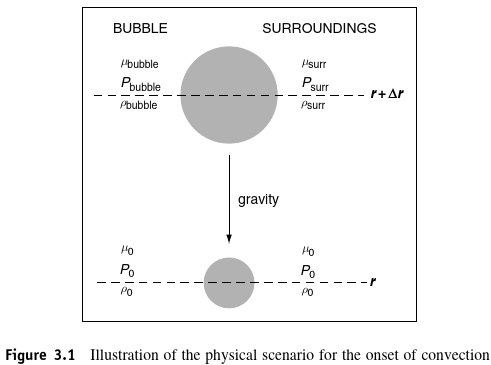
\includegraphics[trim={0cm 0cm 1cm 0cm},clip, keepaspectratio,width=0.99\textwidth]{convectivestability}\label{fig:convectivestability}
\end{figure}

\begin{itemize}
    \item Rayleigh-Taylor instability: $\TDy{r}{\ln{(\mu)}}>0$
    \item $\nrad>\nad-\frac{\xi_{\mu}}{\xi_T}\TDly{(P)}{(\mu)}$
\end{itemize}
		
\subsection{Gradiente ambientale nelle regioni convettive}



\chapter{evolution of stars}
%\PartialToc

\subsection{Massa minima innesco fusione H}

Temperatura minima per innesco idrogeno: $T_{min}\approx\SI{1.5e6}{\kelvin}$
\begin{align*}
&P_c=K_{NR}n_e\expy{5/3}+n_ikT_c=K_{NR}\frac{\rho_c}{m_H}]\expy{5/3}+\frac{\rho_c}{m_H}kT_c\\
&kT_c=A\rho_c\expy{1/3}-B\rho_c\expy{2/3}\\
&kT_{c,max}\propto G^2\frac{m_H\expy{8/3}}{K_{NR}}M\expy{4/3}
\end{align*}

\subsection{Massa massima}

\begin{align*}
&P=P_i+P_e+P_R=\frac{\rho_c}{\mu m_H}kT_c+\frac{1}{3}aT_c^4\\
&P_g=\beta P_c\quad P_R=(1-\beta)P_c
\end{align*}

\subsection{Struttura stellare approssimata}

\begin{itemize}
\item \keyword{Approssimazione zero per $M_r(0)$ e $M_r(R)$}:
Al centro della stella $\TDy{r}{P}=-\frac{GM_r}{r^2}\rho\approx-\frac{4\pi}{3}r^3\rho_c\frac{G}{r^2}\rho_c\approx-\frac{4\pi}{3}rG\rho_c^2$, vicino alla superficie $\TDy{r}{P}\approx-G\frac{M\rho}{r^2}$: se la composizione chimica \'e costante
\begin{align*}
&\TDy{r}{P}\approx-\frac{4\pi}{3}G\rho_c^2r\exp{-r^2/a^2}\\
&P(r)\approx-\frac{2\pi}{3}G\rho_c^2a^2[\exp{-r^2/a^2}-\exp{-R^2/a^2}]
\end{align*}

$4\pi\rho r^2dr=dm$ ci permette di riscrivere equilibrio idrostatico $GM_rdM_r=-4\pi r^4dP$:
\begin{align*}
&\frac{1}{2}GM_r^2=-4\pi\int_0^rr'^4\TDy{r}{P}\,dr\\
&M_r=\frac{4\pi a^3}{3}\rho_c\Phi(x)\quad x=r/a\\
&\Phi(x)=6\int_0^xx'^5\exp{-x'^2}\,dx'\approx x^6-3/4x^8+3/10x\expy{10}+...
\end{align*}
per alta $\rho_x$ $a\ll R$ ...:
\begin{align*}
&M\approx M_r=\frac{4\pi\rho_ca^3}{3}\Phi(\frac{R}{a})\approx\frac{4\pi\rho_ca^3}{3}\sqrt{6}\\
&P_c\approx\frac{2\pi}{3}G\rho_c^2a^2\approx[\frac{\pi}{36}]GM\expy{2/3}\rho_c\expy{4/3}
\end{align*}

\item Politropa $n=3/2$: $P_c\propto M\expy{2/3}\rho_c\expy{4/3}$

\item Politropa $n=3$: $P_c\propto M\expy{2/3}\rho_c\expy{4/3}$

\end{itemize}

\section{Evolution scaling}

\begin{itemize}
    \item \xaumenta{M}, \xdiminuisce{\tau}
    \item \xdiminuisce{M}, \xaumenta{\rho_c}, \xdiminuisce{T_c}
    \item \xaumenta{Z}, \xdiminuisce{L}, \xdiminuisce{T_e}, \xaumenta{\tau}
    \item \xaumenta{Y}, \xaumenta{L}, \xaumenta{T_e}, \xdiminuisce{\tau}
    \item Opacit\'a in funzione di Y: \xaumenta{Y}, \xdiminuisce{\kappa} 
\end{itemize}

\subsection{Low mass star}

tempi evolutivi in HRD


\section{From proto-star to Pre-MS}

\begin{itemize}
\item Isothermal collapse of MC ($t_{cool}\ll t_{ff}$, $P\propto\rho$). MC build up as gas flow into arm's potential well. massa di Jeans $M_J\propto\expy{3/2}\rho\expy{-1/2}$. $M_j$ diminuisce all'aumentare di densit\'a: frammentazione
\item Virial theorem.

\adjm{\rho\TDy{t}{\vec{u}}=-\nabla P-\rho\nabla\phi+\frac{1}{c}\vecp{j}{B}}

\adjm{\rho\TDy{t}{\vec{u}}=-\nabla P-\rho\nabla\phi+\frac{1}{4\pi}(\scap{B}{\nabla})\vec{B}-\frac{1}{8\pi}\nabla|B|^2}

\adjm{\frac{1}{2}\PtwoDy{t}{I}=2T+2U+W+M}

\adjm{I=\int \rho|r|^2\,d^3x,\ T=\frac{1}{2}\int\rho|\vec{u}|^2\,d^3x,\ U=\frac{3}{2}\int nKT\,d^3x=\frac{3}{2}\int P\,d^3x}

\adjm{W=\frac{1}{2}\int\rho\phi\,d^3x\ M=\frac{1}{8\pi}\int|B|^2\,d^3x}

No evidence for collapse of giant complexes: $2T+2U+W+M$.

\adjm{\frac{T}{|W|}\approx\frac{1}{2};\Delta V^2\invers{(\frac{GM^2}{R})}}

\adjm{=0.5(\frac{\Delta V}{\SI{4}{\kilo\meter\per\second}})^2(\frac{M}{10^5\msun{}})\expy{-1}(\frac{R}{\SI{25}{\parsec}})}

\adjm{\Delta V\approx\sqrt{\frac{GM}{R}}=V_{vir},\ t_{ff}\approx\sqrt{\frac{R^3}{GM}}}

Small clumps moving moving in gravitational field of whole ensamble.
\item Denser regions with point IR source. (Fase adiabatica $P\propto\rho\expy{\gamma}$, $T\propto\rho\expy{2/3}$ per mono-ideal gas) Inner region of collapsing cloud becomes denser/optically thicker (first core formation $\tau\approx\SI{1.5e7}{\year}$): role of ambipolar diffusion. Typical mass $M_*=\num{e-2}\msun{}$, $R_*=\SI{5}{\astronomicalunit}$, $\rho\approx\SI{e-10}{\gram\per\cubic\cm}$. Energy radiated by denser core is absorbed by free-falling gas and re-emitted in IR
\item The first core of molecular hydrogen collapse as soon as T is raised enough to begins molecular dissociation (for $T>2000K$ we have collisional diss)
\begin{align*}
&0=-\frac{1}{2}\frac{GM_*^2}{R_*}+\Delta E_{int}+L_{rad}t\\
&L_{rad}\approx L_{acc}=\frac{\dot{M}GM_*}{R_*}\\
&\Delta E_{int}=\frac{XM_*}{m_H}[\frac{\Delta E_{dis}(H)}{2}+\Delta E_{ion}(H)]+\frac{YM_*\Delta E_{ion}(He)}{4m_H}
\end{align*}
\item Birthline
\begin{align*}
&\tau_{KH}=\frac{GM_*^2}{R_*L_*}\propto L_*\expy{-3/2}\\
&\TDy{t}{R_*}\propto-\frac{R_*}{t_{KH}}\\
&L_*=4\pi\sigma T_*^4R_*^2\\
&\TDy{t}{L_*}\propto-\frac{L_*}{\tau_{KH}}
&T_*\approx\const{}
\end{align*}
The most luminous therefore youngest object reflect its nature of accreting object within collapsing dense core: surface temperature and luminosity are set by infall (\numrange{e-5}{e-6}$\msun/yr$) dynamics (expected to change when infall end), radius by internal structure and is the same for protostar and pre-MS star; the birthline is the locus of pre-MS star with protostellar radii. At $M_*=8\msun$ the birthline intercept the ZAMS
\item Slower accretion give radius more time to shrink but D-burning thermostat limit that. D ignition: $^2H+^1H\to^3He+\gamma(\SI{5.5}{\mega\ev})$.
\item ''position'' of Hayashi track: \xaumenta{Y}, \xaumenta{T_e}; \xaumenta{Z}, \xdiminuisce{T_e}; \xdiminuisce{M}, \xdiminuisce{T_e}
\item formation of radiative core caused by \xdiminuisce{R}, \xdiminuisce{L}, \xdiminuisce{\nabla_{rad}} ($L\propto R^2$); parallelamente \xdiminuisce{R}, \xaumenta{T}, \xdiminuisce{\exv{\kappa}} ($\kappa_{kr}\propto$), \xdiminuisce{\nrad{}}, \xaumenta{T_e}
(stahler palla fig 16.8)
\end{itemize}

\subsection{Pre-MS star model}
Structure equation:
\begin{align*}
&\PDy{M_r}{r}=\frac{1}{4\pi r^2\rho}\\
&\PDy{M_r}{P}=-\frac{GM_r}{4\pi r^4}\\
&\PDy{M_r}{L_{int}}=\epsilon-T\PDy{t}{s}
\end{align*}
fourth equation in radiative/convective zones
\begin{align*}
&T^3\PDy{M_r}{T}=-\frac{3\kappa L_{int}}{256\pi^2\sigma r^4}\\
&\PDy{M_r}{s}
\end{align*}
HE integrated from phot to inf
\adjm{P_{phot}=\frac{GM_*}{R_*^2}\int_{R_*}^{\infty}\rho\,dr\approx\frac{GM_*}{R_*^2\kappa_{phot}}\int_{R_*}^{\infty}\rho\kappa\,dr=\frac{GM_*\Delta\tau}{R_*^2\kappa_{phot}}}
(adim eqs:
\adjm{x=\frac{r}{R},\ q=\frac{M_r}{M},\ t=\frac{T}{T_0},\ p=\frac{P}{P_0},\ T_0=\frac{\mu GMm_H}{Rk},\ P_0=\frac{GM^2}{4\pi R^4}}
Continuity: $\TDy{x}{q}=\frac{p}{t}x^2$, HE: $\TDy{x}{p}=-\frac{p}{t}\frac{q}{x^2}$, $\nad$ for fully convective star: $P=CT\expy{5/2}\to p=Et\expy{2.5}$ (C determines the adiabat).
HayT is vertical $\TDly{T_e}{L}>10$, mild mass deps $\TDly{M}{T_e}\approx0.2$. Realistically: surface condition+super-adibat layer.
)

As T increses due to contraction (V.T.)a central radiative core is formed: when a sizeble radiative core formed path toward higher $T_e$ is almost horizontal.
At temperature \SIrange{1e6}{2.5e6}{\kelvin} D/Li(Be/B) are burnt by proton capture (Li/D depletion at surface for fully convective star).
In general larger masses have lower Li depletion, given mass increases increasing Z: \xaumenta{M}(or \xdiminuisce{Z}) lower convective zone but also earlier retreat from center (fig 16.10)


\section{Sequenza principale}

\section{From H central exhaustion to He central ignition: overall contraction/TO to TRGB}

\subsection{Low mass stars ($M_{cSC}\approx0.1\msun$)}

\begin{itemize}
\item As H exhausts in center $T_M$ moves outward: at TO $90\%$ of H-burning in thick shell of $0.2\msun$: H-burning shell becomes thinner and thinner as CNO is strongly T-dep and as H-depleted inside and T drops in envelope.
\end{itemize} 

\end{document}

\stopcontents[chapters]
\end{document}